\section{Approach}

\subsection{B and B+ Backend}
Our approach to creating the backend which would handle the structure
of the trees and their contents was fairly straight forward.  We had
access to well defined rules that define B and B+ trees so designing
the general structure of the trees was simple enough.  However, since
our intent was for the web interface to be able to actively switch
between B and B+ tree representations, we had to factor in as much
shared resources as we could to assist in the process of switching
between the two tree types.  Conveniently, B and B+ trees are fairly
similar, so it did not take much extra effort to make much of the
trees structure shared.  Specfically, both tree types utilize the
same node/block object we have created.  While the nodes have some
properties unique to either type of tree, which comes at a slight
memory cost, it makes it easier to switch back and forth.  We also
keep a master list of all values in the tree at any given time.  This
master list is the primary element that allows us to switch between
tree structures.  Whenever we want to switch, we simply copy the
element list, change the tree type, and then insert every value into
the tree, in the same order they had been inserted into the previous
tree.  It should be noted that this method could result in getting a
different tree if you switched from B tree to B+ and back again, or
vice versa.  this is because we do not execute all operations that
occurred on the previous tree, just insertions of values that were in
it, so any imperfect organization caused by deletion could be cleaned
up by switching back and forth between tree structures.  While
structurally the trees have various commonalities, the methods of
insertion, deletion, and searching the trees still had to remain
completely separate due to the subtly differences in the tree
structures.

\subsection{HTML5 Frontend}
Due to the dynamic nature of the content we needed to display to the
user, we decided to use the HTML5 \texttt{canvas} element. With the
\texttt{canvas} element, it is possible to draw things directly on the
screen. However, the \texttt{canvas} element is quite low level in
its functionality. In order to utilize higher order abstractions, we
utilized a library called \textit{Kinetic.js}. This library allowed us
to specify groups of shapes which would be considered as a consistent
whole when moving across the screen. From this we could construct node
and edge objects which would be consistent throughout the modeling
process.

User input occurs through the use of text boxes and buttons directly
underneath the \texttt{canvas} display. These buttons are labeled with
the different possible actions: insert, delete, and search. By
inputting a value into the associated text box, and pressing the
button, the user initiates a modification to the tree.

%% \begin{figure}[htp]
%% \centering
%% 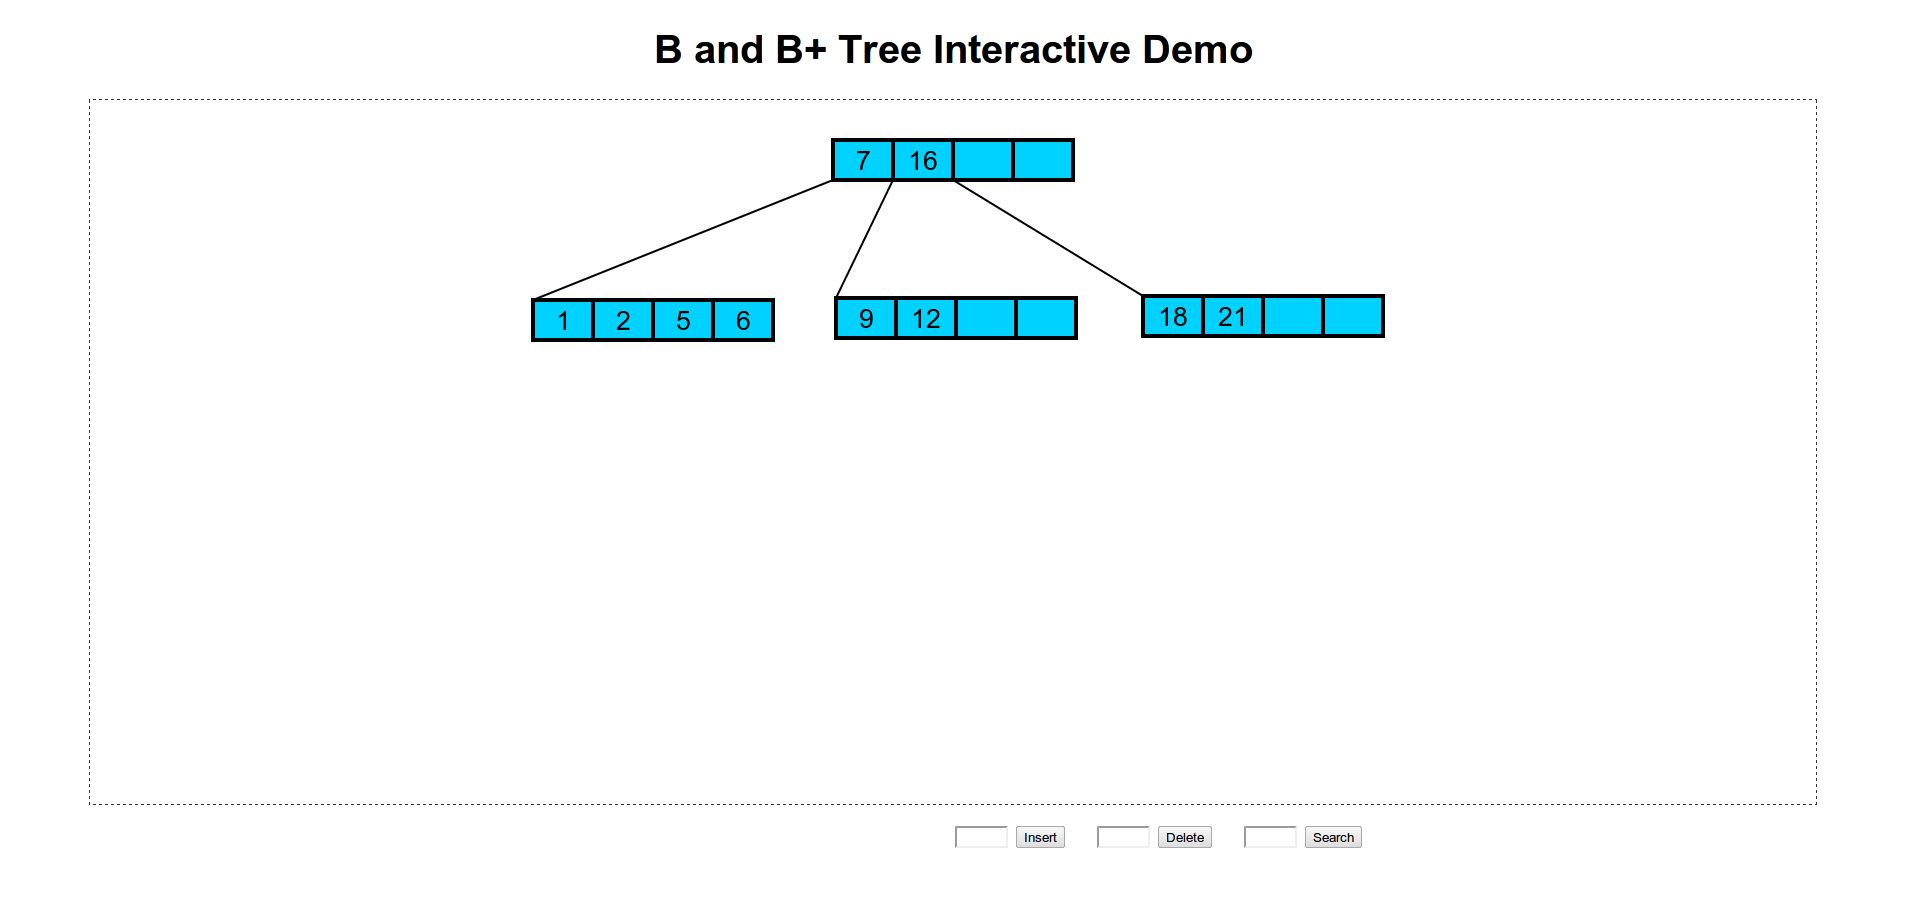
\includegraphics[scale=0.25]{images/Interface.png}
%% \caption{The user interface of our project}
%% \label{UI}
%% \end{figure}
